% Chapter Template

\chapter{Results} % Main chapter title

\label{Chapter3} % Change X to a consecutive number; for referencing this chapter elsewhere, use \ref{ChapterX}

%----------------------------------------------------------------------------------------
%	SECTION 1
%----------------------------------------------------------------------------------------
\section{Setup}
In this paper, we discussed a pipeline implemented using python then with C\# and Unity's real time development platform as the visualization engine. We ran a FDS simulation set to output plot3D every 0.5 seconds a 20m x 20m x 20m mesh containing voxels  0.2m x 0.2m x 0.2m  in size, with open boundary conditions. The simulation was 100 seconds in length with a ground fire igniting 10 seconds in to the simulation, with a wind  of 5.6 m/s originating from the south west (215\textdegree) and trees evenly distributed on the mesh. [Figure \ref{fig:CFDTopDown} show a top down view of our visualization rendered in SmokeView] \par
\section{Analyses}
The total run time for this simulation was  \color{red}510 \color{black} minutes to complete, running 4 cores of an i7 4790k in parallel, while calculations we disused in this paper were able to complete in \color{red} 15 \color{black} minutes,with no parallelization at the moment. Additionally the size of the CFD output files was 5.0 GB while the saved data needed for full Virtual Reality using our methodology is 28.9 MB  a 99.4\% reduction in file size. The use of unity's development platform allows us to compile and the possibility to make available for distribution a self contained system to help improve training for fire fighters.

\begin{figure}
\centering
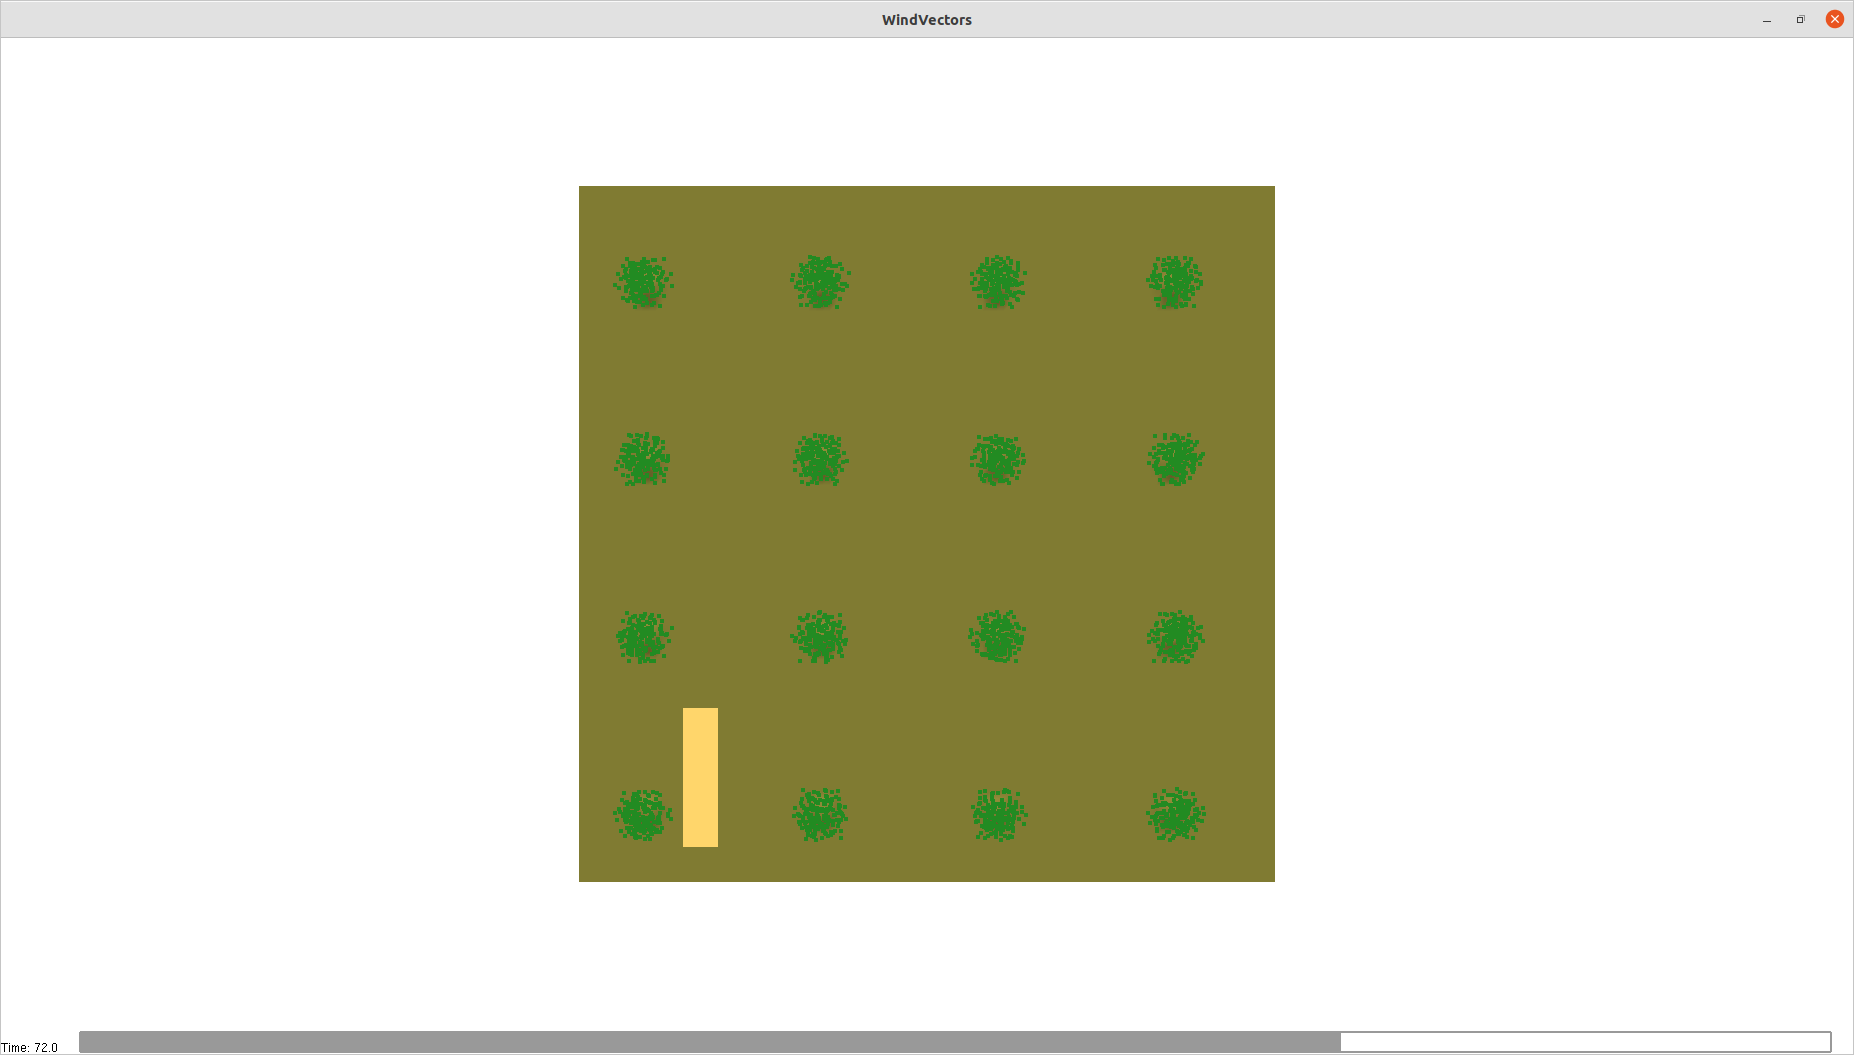
\includegraphics[scale=.1]{Figures/fdsPartTopView.png}
\decoRule
\caption[CFD Simulation]{A top-down view of the CFD simulation}
\label{fig:CFDTopDown}
\end{figure}